% Chapter 7
\chapter{Handheld Tendon-Driven Surgical Instrument: Design, Packaging and Control}

\label{Chapter7}

\begin{chaptersummary}
This chapter presents a complementary application case within the tendon-driven mechanism framework of the thesis: a compact handheld laparoscopic instrument. The instrument is positioned alongside Lasso Gripper rather than as a derivative of it. Whereas Lasso Gripper serves as the primary novel mechanism platform of the thesis, the handheld instrument demonstrates how the same tendon-driven design variables can be organized in a more constrained engineering context: compact packaging, repeatable bidirectional cable motion, ergonomic handheld operation, safety, and clinically practical distal dexterity. The chapter first introduces these primary design objectives and then describes the overall system architecture connecting proximal actuation, paired-cable reel mechanisms, cable routing and guidance structures, interchangeable end-effectors, and the input/HMI subsystem.

The mechanical and electromechanical implementation is subsequently detailed, including actuator selection and arrangement, paired-cable winding mechanisms, cable routing strategies, tip interfaces and quick-swap designs, encoder-integrated input modules, and compact packaging considerations. Particular emphasis is placed on minimizing hysteresis, preserving cable tension, reducing distal inertia, and maintaining reliable force transmission within the spatial constraints of handheld surgical instrumentation.

The chapter further presents the control architecture of the system, including the modeling framework, Denavit-Hartenberg coordinate definitions and forward kinematics, overall system architecture and data flow, encoder-based intent estimation and command mapping, low-level position and tension control loops, firmware communication, and human-machine interaction design. Safety-related procedures such as homing, fault handling, and tension-release logic are also discussed as integral components of the instrument's operational reliability.
\end{chaptersummary}

\section{Necessity of Developing a Handheld Motorized Medical Instrument}
The handheld surgical instrument is developed as a complementary application case within the tendon-driven mechanism framework introduced in this thesis. Whereas Lasso Gripper uses an unconstrained tensile loop to achieve adaptive capture, the present system uses guided cable transmission to achieve compact distal dexterity and repeatable control. The relationship between the two systems is therefore not that one directly originates from the other. Instead, both are built on controlled tension, proximal actuation, and flexible transmission, while serving different roles in the thesis. Lasso Gripper forms the main mechanism innovation, and the handheld instrument provides a secondary engineering implementation that applies the same design language to a medical-device setting.

Contemporary research in surgical robotics has predominantly prioritized maximizing tip-positioning accuracy through advanced actuation methods and the integration of supplementary sensors. While these approaches demonstrably enhance precision, they often overlook a critical practical constraint: the weight-to-functionality ratio. The evident correlation between enhanced capabilities achieved through more powerful motors or additional sensing and increased instrument mass creates a significant adoption barrier. This added weight often leads surgeons to favor simpler, nearly weightless traditional instruments over their motorized counterparts, despite the latter's technological advantages.

To resolve this fundamental trade-off, the present work introduces a holistic approach to ergonomic and functional design in robotic-assisted surgery. This chapter frames the surgical instrument as a complementary, application-driven embodiment of the tendon-driven mechanism thesis: instead of proposing a new capture principle as in Lasso Gripper, the objective here is to maximize distal dexterity and control fidelity while preserving low mass and practical usability. The proposed system embodies a dedicated effort to distribute system components intelligently, minimize inertial load, and integrate multi-modal sensing without compromising the manipulator's agility or the surgeon's comfort.


\section{Core Design Advantages for Handheld Applications}

This cable-driven, differential actuation philosophy offers several fundamental advantages that are particularly suited to the development of advanced handheld devices:

\begin{itemize}
\item \textbf{Enhanced Dexterity and Manipulation}: The system enables multi-degree-of-freedom manipulation (e.g., rotation, twisting) using a minimal number of actuated elements. This is crucial for applications requiring fine motor control within confined spaces.

\item \textbf{Inherent Compliance and Safety}: The system is naturally compliant. Cables under tension provide a direct force-feedback path. If an unexpected obstacle is encountered, the cables will slacken rather than apply a rigid, potentially damaging force. This passive safety feature is a critical asset for interactions in unstructured or delicate environments.

\item \textbf{Proximal Actuation and Minimal End-Effector Mass}: A primary benefit for handheld device design is the ability to locate the heavy actuators (motors) and associated drive electronics proximally, either in the device's handle or even in a remote unit. This dramatically reduces the mass and inertia of the distal end-effector, leading to improved ergonomics, reduced user fatigue, and the potential for higher maneuverability and smaller form factors at the interaction point.
\end{itemize}

\section{Defining Performance Metrics for Structural Design}

To translate this conceptual framework into a viable product, key performance metrics must be established. These metrics represent the surgical-domain counterpart within the same tendon-driven design space: instead of capture range and adaptive loop closure, the emphasis here shifts to precision, low hysteresis, compact routing, and stable bidirectional tension transmission. They will directly guide the structural design choices detailed in the next section:

\begin{itemize}
\item \textbf{Precision and Resolution}: The minimum achievable incremental movement of the end-effector tip, targeting sub-millimeter and sub-degree accuracy for delicate tasks.

\item \textbf{Force Capability}: The maximum tensile force the cables must transmit to securely grasp and manipulate objects of a target weight range.

\item \textbf{Range of Motion}: The required angular deflection and rotational range of the end-effector to perform its intended functions effectively.

\item \textbf{Force Transmission Efficiency}: Minimizing friction losses throughout the cable drive path is essential for accurate force feedback and predictable control.

\item \textbf{Low Hysteresis and Backlash}: The structural design must ensure minimal play and elastic deformation in the system to guarantee precise, repeatable, and immediate response to actuator inputs.
\end{itemize}

\section{Pathway to Structural Implementation}
The structural implementation is based on the same tendon-driven mechanism variables examined throughout the thesis: compliance, proximal actuation, differential control, routing geometry, and explicit tension management. In the handheld surgical instrument, these variables are configured for stricter constraints on packaging, repeatability, sterilization feasibility, and operator ergonomics.

The next section addresses the critical task of transforming this mechanism framework into a robust mechanical reality. The structural design must meticulously integrate several key subsystems:
\begin{enumerate}
    \item \textbf{Actuation Unit Selection and Layout}: Choosing motors and sensors that meet the performance metrics and determining their optimal arrangement.

    \item \textbf{Cable Routing and Guidance System}: Designing low-friction, precise pathways for the cables to ensure efficient force transmission and longevity.

    \item \textbf{End-Effector Configuration and Cable Termination}: Engineering the interface where the cables attach to the manipulator, ensuring secure anchoring, precise motion, and mechanical advantage.

    %\item \textbf{Ergonomic Handle and Housing Design}: Packaging the system into a form factor that is balanced, comfortable, and intuitive for the user to hold and operate over prolonged periods.
\end{enumerate}


Through this structured approach, the subsequent design shows how the shared tendon-driven mechanism framework can produce a functional cable-driven surgical instrument under medical-device constraints. Rather than treating the handheld instrument as a derivative of Lasso Gripper or as an isolated engineering project, this thesis positions it as a complementary application case under the same mechanism-level theme. Lasso Gripper remains the main exploratory contribution, focused on tendon-driven adaptivity and loop-based capture in an open manipulation setting. The surgical instrument is secondary and application-oriented, focused on guided cable routing, compact packaging, and controllability in a tightly constrained medical setting. Emphasizing this relationship keeps the thesis focused on tendon-driven mechanisms without overstating a direct innovation transfer from one device to the other.

\section{Mechanism and Design}
\begin{figure}[htbp]
    \centering
      \begin{subfigure}[b]{\linewidth}
        \centering
        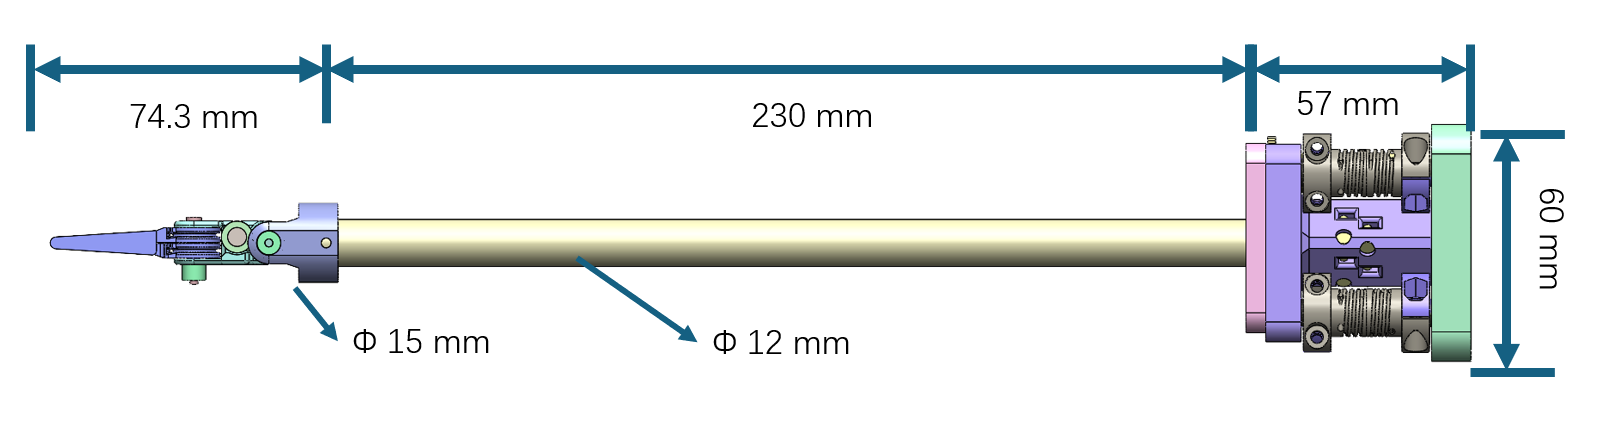
\includegraphics[width=\linewidth]{Figures/Chapter4/Winding_Size.png}
        \caption{Shaft and winding dimensions}
    \end{subfigure}

    \vspace{0.5em}

    \begin{subfigure}[b]{\linewidth}
        \centering
        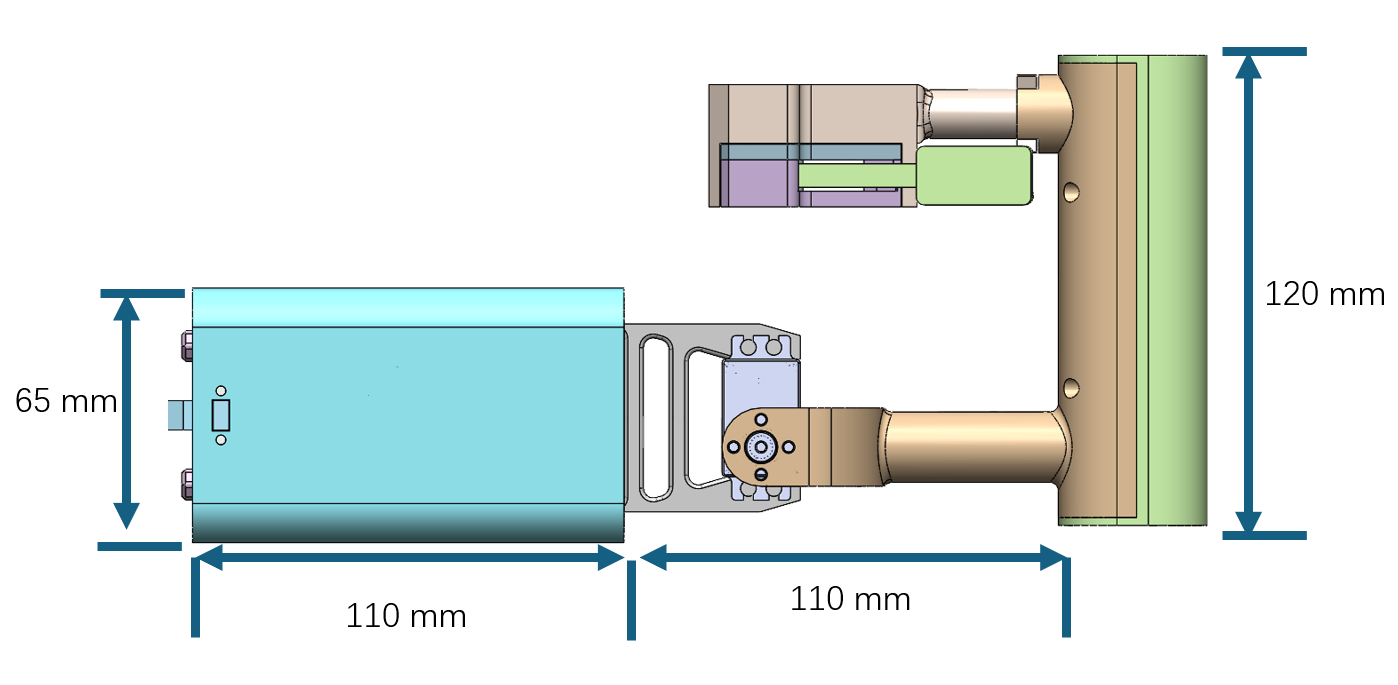
\includegraphics[width=\linewidth]{Figures/Chapter4/Main_Frame_Size.png}
        \caption{Main dimensions}
    \end{subfigure}
    \caption{Overall mechanical layout of the handheld tendon-driven instrument. The design separates the handheld actuation and control housing from the distal tool module so that the mass of motors and electronics is concentrated proximally, while the cable-driven tip remains compact.}
    \label{fig:main_frame_exploded}
\end{figure}

The system is organized into three physical modules: the proximal main frame, the cable-driven shaft and winding assembly, and the distal interchangeable tool. This modular arrangement follows the same proximal-actuation principle underlying the tendon-driven mechanism framework of this thesis, but adapts it to the stricter requirements of handheld surgical instrumentation. The main frame contains the higher-mass actuators, control board, and input interface; the shaft transmits cable tension through a guided internal route; and the distal tip converts cable displacement into multi-degree-of-freedom tool motion.

The total prototype mass is approximately 682\,g. Of this, the handheld body accounts for about 539\,g and the distal operating forceps account for about 143\,g. Concentrating most of the mass in the handle reduces the inertia of the distal portion and makes the device easier to orient during fine manipulation. The main frame measures approximately 110\,mm by 65\,mm in the motor housing region, while the distal shaft assembly uses a 250\,mm carbon tube with a 12\,mm outer diameter and a 15\,mm proximal coupling region. These dimensions were selected to balance compactness, cable routing clearance, and sufficient stiffness for hand-guided use.

\begin{table}[htbp]
    \centering
    \caption{Mass distribution of the handheld instrument prototype}
    \label{tab:mass_distribution}
    \begin{tabular}{p{0.23\linewidth} c p{0.48\linewidth}}
        \toprule
        Module & Mass & Design implication \\
        \midrule
        Handheld body & 539\,g & Motors, electronics, input interface, and main housing \\
        Operating forceps & 143\,g & Distal tool and shaft kept lighter to reduce manipulation inertia \\
        Total prototype & 682\,g & Bench-top handheld validation platform \\
        \bottomrule
    \end{tabular}
\end{table}

\subsection{Output Motors}
A key challenge for handheld cable-driven devices is selecting actuators that combine low mass with sufficient torque. The chosen output actuator, the Feetech STS3032 smart servo, offers a favorable torque-to-volume ratio and built-in low-level drive electronics useful for closed-loop control. It weighs approximately 20.6\,g, measures $23 \times 12 \times 27.5\,\mathrm{mm}$, and provides a stall torque of about $4.5\,\mathrm{kg\,cm}$, enabling reliable tensioning through small-diameter pulleys.

The four STS3032 servos are assigned to the output-side tool motions, including roll, pitch, yaw, and gripper opening/closing. Their serial-bus communication simplifies wiring and supports daisy-chaining, which reduces the number of conductors inside the handle and aids miniaturization. As smart servos, they can be commanded at the level of position and speed while also reporting state variables such as position, speed, load, voltage, temperature, and current. This low-level feedback allows the controller to implement repeatable position commands, monitor loading, and protect the cable drive from excessive tension.
\subsection{Input Motors and Sensors}

The control philosophy for this cable-driven handheld device is based on replicating the user's hand movements with high fidelity and translating them into precise motions of the distal end-effector. This requires a sophisticated input system that can accurately capture the intent of the user's fingers while providing sufficient force feedback and stability.


\begin{figure}[htbp]
    \centering
    \begin{subfigure}[b]{0.45\linewidth}
        \centering
        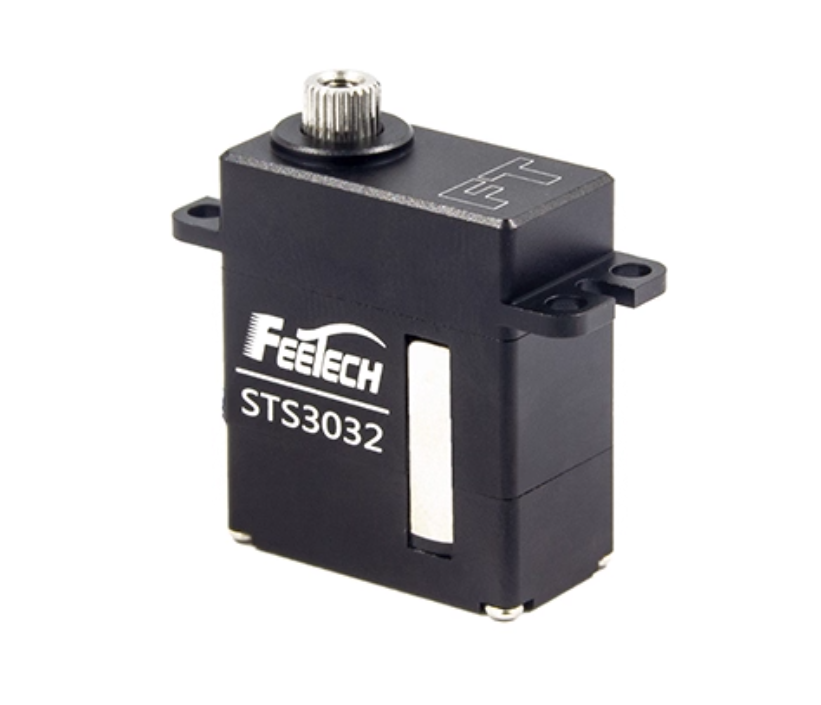
\includegraphics[width=\linewidth]{Figures/STS3032.png}
        \caption{Feetech 3032 for output}
        \label{fig:81}
    \end{subfigure}
    \hfill  % 水平填充，使两张图之间有空隙
    \begin{subfigure}[b]{0.45\linewidth}
        \centering
        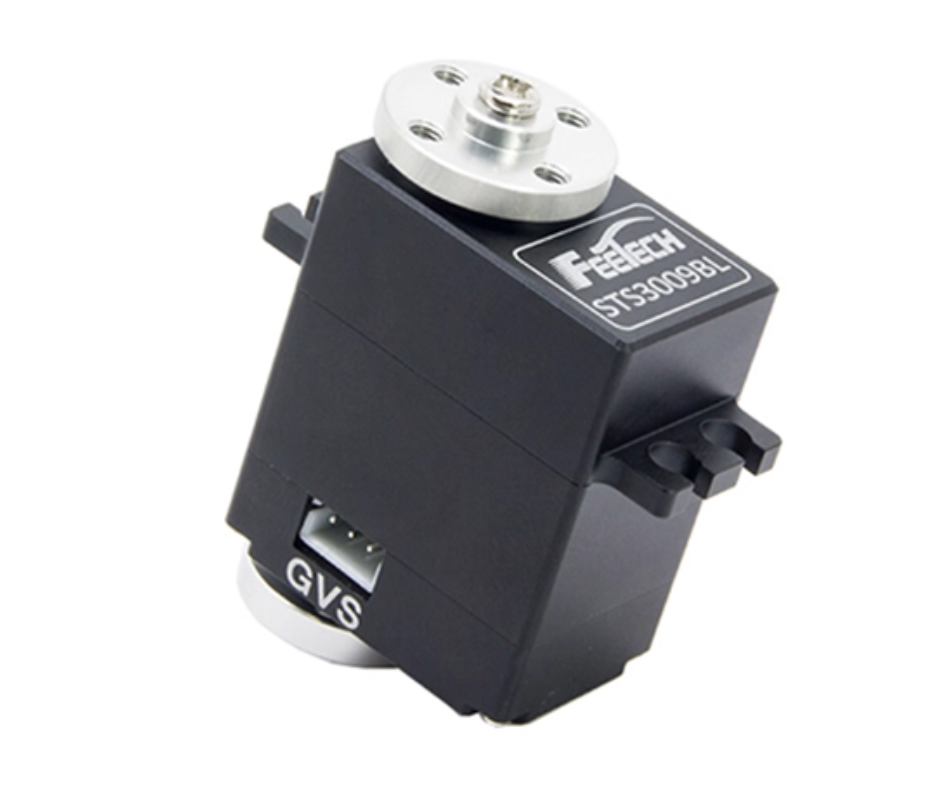
\includegraphics[width=\linewidth]{Figures/STS3009.png}
        \caption{Feetech 3009 for wrist inputs}
        \label{fig:82}
    \end{subfigure}
    \caption{Feetech servos: left motor for output (STS3032), right motor for wrist inputs (STS3009)}
\end{figure}

For the input actuation, shown in Fig.\ref{fig:81}, the Feetech STS3009 servo was selected based on a different set of requirements. Weighing approximately 45\,g, measuring $20 \times 30 \times 36.5\,\mathrm{mm}$, and providing a stall torque of about $11.5\,\mathrm{kg\,cm}$ ($\approx 1.13\,\mathrm{N\,m}$), this larger motor serves two essential functions in the input stage: it maintains mechanical equilibrium by resisting forces from the output tendons, thus offering a stable and responsive feel to the operator, and it helps filter out high-frequency physiological tremors or unintended jerks, ensuring that only deliberate commands are transmitted to the end-effector.


However, since the two input motors alone cannot fully capture all nuanced finger movements, a hybrid sensing strategy was implemented. The two STS3009 servos correspond to the input-side pitch and yaw axes. Two AMS AS5600 magnetic rotary encoders were integrated into the input mechanism to directly detect the remaining roll and open/close commands. These sensors provide 12-bit contactless angular sensing, enabling precise recognition of the pinching gesture of the index finger and thumb, which controls grasping, and the rotational movement of the fingers, which is translated into in-plane rotation of the end-effector. This combination of robust actuation and high-resolution sensing creates an intuitive and stable human-machine interface suitable for delicate manipulation tasks.

\begin{table}[htbp]
    \centering
    \caption{Actuator and sensor allocation in the handheld instrument}
    \label{tab:actuator_allocation}
    \small
    \setlength{\tabcolsep}{3pt}
    \begin{tabular}{@{}p{0.21\linewidth} p{0.09\linewidth} p{0.10\linewidth} p{0.16\linewidth} p{0.34\linewidth}@{}}
        \toprule
        Component & Quantity & Mass & Stall torque & Assigned function \\
        \midrule
        Feetech STS3032 & 4 & 20.6\,g & $4.5\,\mathrm{kg\,cm}$ & Output-side roll, pitch, yaw, and open/close control \\
        Feetech STS3009 & 2 & 45\,g & $11.5\,\mathrm{kg\,cm}$ & Input-side pitch and yaw sensing/stabilization \\
        AS5600 encoder & 2 & -- & -- & Input-side roll and open/close sensing \\
        \bottomrule
    \end{tabular}
\end{table}

\section{Cable Routing and Guidance System}
\subsection{Tip Design}
\begin{figure}[htbp]
    \centering
    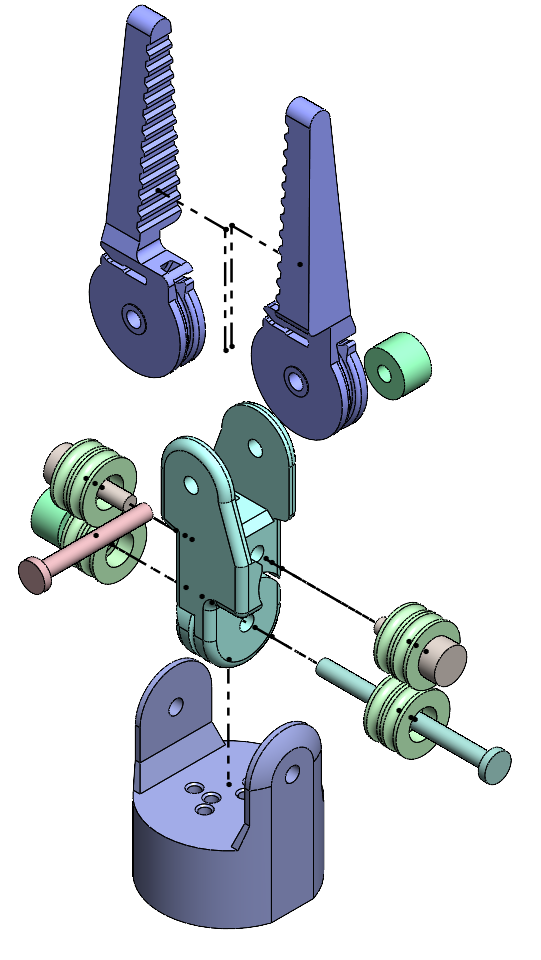
\includegraphics[width=0.5\linewidth]{Figures/Chapter4/Tip_Explode_View_Isometric.png}
    \caption{Exploded view of the distal tip assembly, including the jaw components, middle base, guide pulleys, pivot shafts, and base housing.}
    \label{fig:tip_exploded}
\end{figure}
In addition to motor performance, the accuracy and repeatability of the end-effector's motion are highly dependent on precise cable guidance and sustained tension control. To ensure consistent behavior during operation, each cable must be constrained to move freely yet securely within a meticulously designed path, minimizing unwanted friction and slack.

A specialized tip assembly has been developed to fulfill these requirements. As shown in Fig.~\ref{fig:tip_exploded}, the four cables are routed through custom-machined channels and pulley-like guides before terminating at the moving jaw components. These channels ensure that the cables remain aligned throughout the entire range of motion, avoiding cross-interference and reducing wear.

The two jaw components (fabricated in blue) are mounted onto a central middle base (green). To further enhance cable stability and minimize friction, donut-shaped guides machined via CNC (light green) are integrated into the middle base. These guides act as low-friction directional pulleys, maintaining cable position with high precision and reducing bending stress, thereby extending cable service life.

The main base housing (deep blue) is designed with precision-aligned holes that direct the cables perpendicularly toward the motors. This alignment is critical for maximizing force transmission efficiency and eliminating off-axis loading, which can introduce positioning errors and reduce system responsiveness.

The selected cable is a 7$\times$37 tungsten wire cable with a diameter of 0.5\,mm. It consists of seven braided strands, each composed of 37 fine wires, giving the cable sufficient flexibility for small-radius routing while maintaining a rated breaking force of 501.7\,N. The working cable length is approximately 350\,mm and is constrained by the current winding assembly, which uses a 250\,mm carbon tube as the main shaft structure. A Teflon guide tube is placed inside the carbon tube to reduce sliding friction and prevent metal-to-carbon abrasion. At the distal tip, integrated pulleys guide the cable around direction changes and reduce localized bending stress.

Through this integrated approach--combining dedicated guiding channels, pulley-supported direction changes, and perpendicular alignment--the system achieves high repeatability, reduced hysteresis, and smoother force transmission, making it suitable for delicate manipulation tasks requiring fine motor control.

\subsubsection{Finite Element Analysis of Tip Components}
\label{sec:tip_fea}
To validate the structural integrity of the distal tool assembly, finite element analysis (FEA) simulations were conducted on the two primary load-bearing components: the jaw/tip component and the middle base. The analysis used 6061-T4 aluminum alloy with an elastic modulus of $69{,}000\,\mathrm{N/mm^2}$, Poisson's ratio of 0.33, and a yield strength of $227.53\,\mathrm{N/mm^2}$. The global mesh size was set to 1.5\,mm, and local mesh control of 0.5\,mm was applied near the load and contact regions to better resolve stress concentrations around the cable-contact and pivot features.

The applied loads were derived from the STS3032 stall torque and therefore represent conservative worst-case loading rather than continuous normal operation. In normal use, firmware-level position, speed, and load limits prevent sustained stall operation; nevertheless, checking the components against a stall-torque-derived case provides a useful structural upper bound for the prototype.

\begin{figure}[htbp]
    \centering
    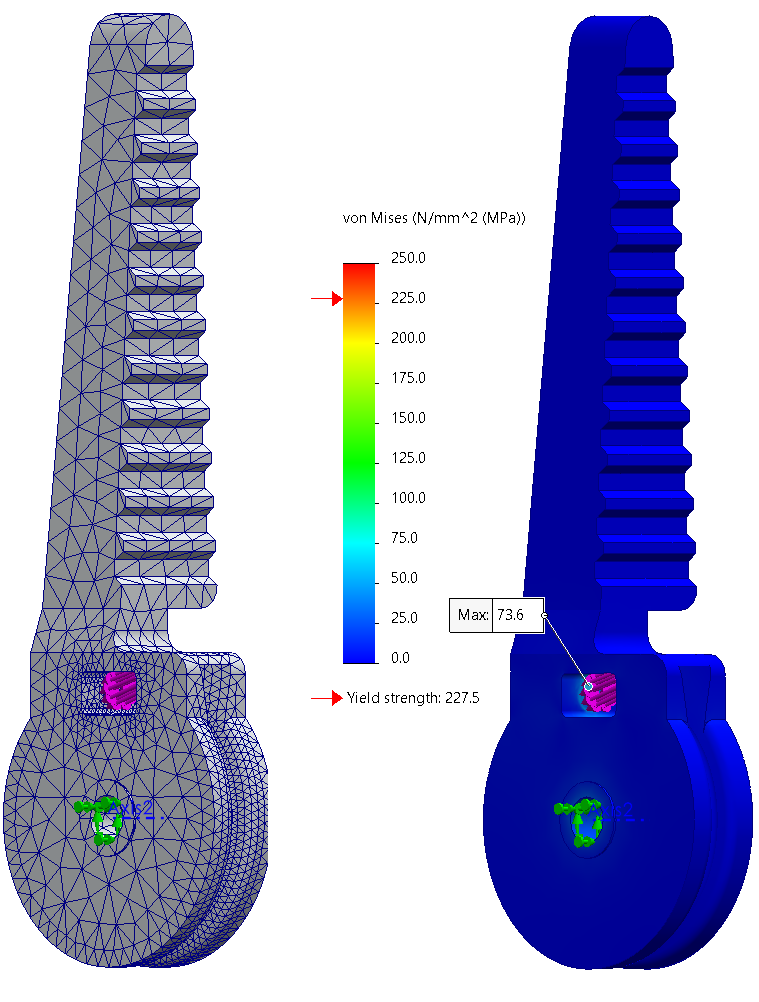
\includegraphics[width=0.7\linewidth]{Figures/Chapter4/Tip_Mesh_FEA.png}   
    \caption{FEA setup and von Mises stress result for the jaw/tip component under the stall-torque-derived loading condition.}
    \label{fig:tip_fea_new}
\end{figure}

\paragraph{Jaw/tip FEA}
The jaw/tip component was constrained at the pivot region and loaded at the cable-contact region according to the worst-case cable tension estimated from the STS3032 stall torque. The maximum von Mises stress was $73.6\,\mathrm{MPa}$, as shown in Fig.~\ref{fig:tip_fea_new}. Compared with the 6061-T4 yield strength of $227.53\,\mathrm{MPa}$, the corresponding safety factor is approximately
\[
SF_{tip}=\frac{227.53}{73.6}\approx 3.09 .
\]
This indicates that the jaw/tip component remains below yield under the conservative load case.

\begin{figure}[htbp]
    \centering
    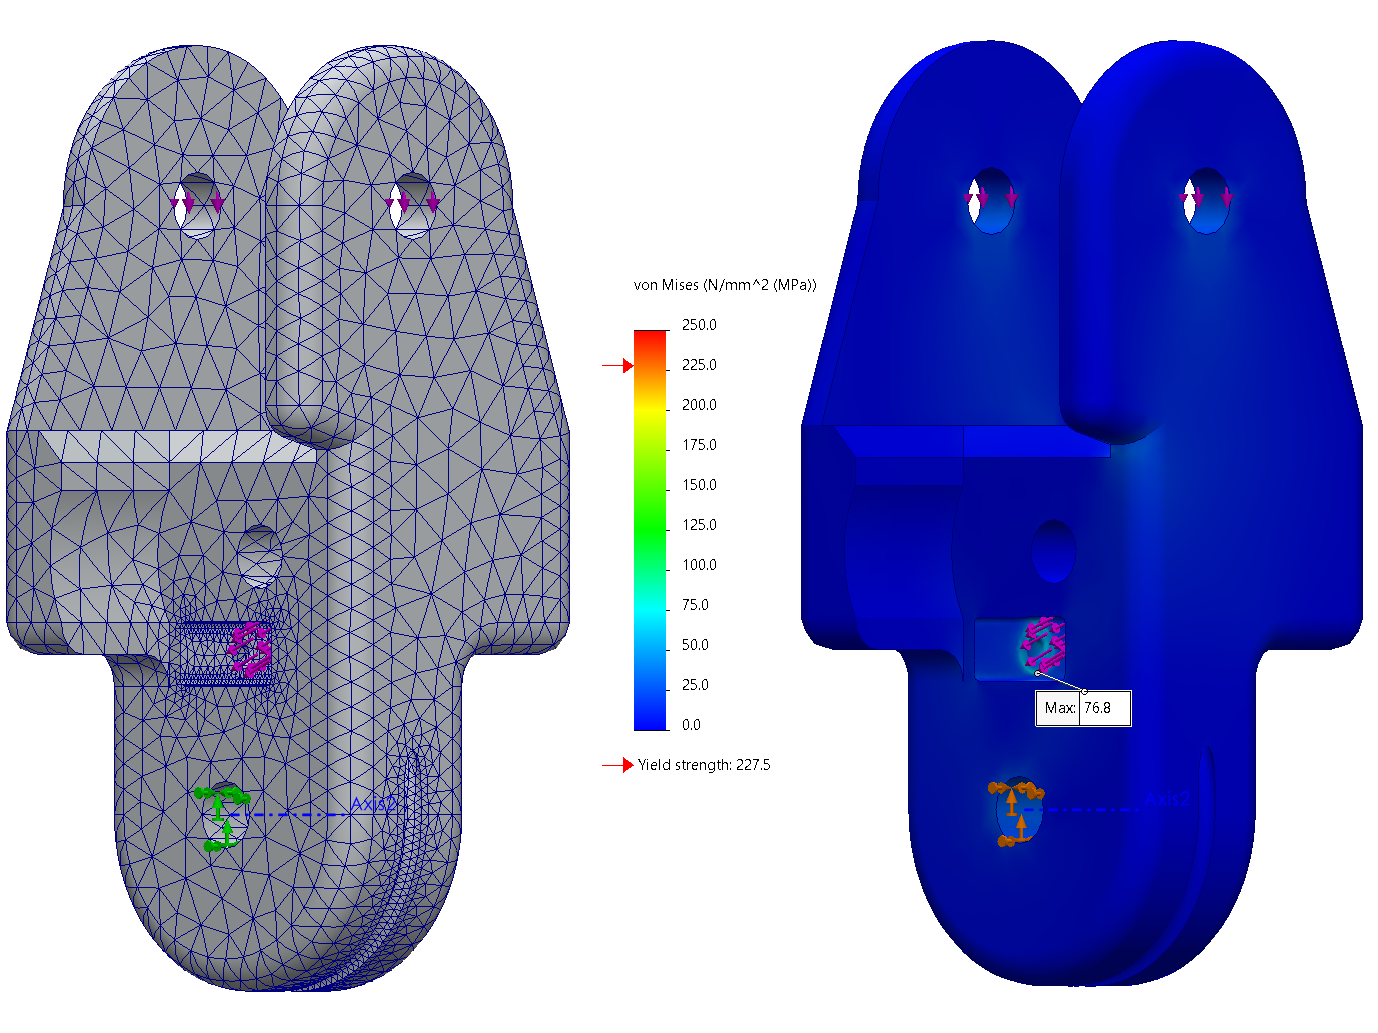
\includegraphics[width=0.9\linewidth]{Figures/Chapter4/Mid mesh&FEA.png}
    \caption{FEA setup and von Mises stress result for the middle base. The load case includes the cable-induced load and the extreme double downward forces transmitted from the tip.}
    \label{fig:mid_fea_new}
\end{figure}

\paragraph{Middle base FEA}
The middle base was evaluated under a combined loading case. In addition to the cable-induced load, the model includes the extreme double downward forces transmitted from the two tip/jaw components, representing a conservative condition in which both jaws transfer load into the base simultaneously. The maximum von Mises stress was $76.8\,\mathrm{MPa}$, as shown in Fig.~\ref{fig:mid_fea_new}. The corresponding safety factor is
\[
SF_{mid}=\frac{227.53}{76.8}\approx 2.96 .
\]
The result confirms that the middle base also remains below the yield strength under the combined extreme loading condition.

Overall, the updated FEA results indicate that both the jaw/tip and middle-base components have sufficient static strength for prototype validation under the conservative stall-torque-derived loading cases. The highest stresses appear near load introduction and geometric transition regions, so future design iterations should continue to use local fillets, adequate wall thickness around guide features, and careful deburring to reduce stress concentration and cable wear.
\subsection{Reel}

A fundamental challenge in cable-driven mechanisms lies in maintaining adequate tension during both winding and unwinding phases. In a conventional single-motor-single-cable configuration, unidirectional actuation presents a significant limitation: while rotation in one direction (e.g., clockwise) effectively pulls and tensions the cable, reverse rotation (counterclockwise) does not positively push the cable but often results in slack accumulation along the path. This leads to unpredictable response, reduced positional accuracy, and potential entanglement.

To address this issue, a paired-cable design has been implemented. The two cables corresponding to a single degree of freedom are affixed to the same axial shaft driven by one motor. This configuration effectively reforms the two independent cables into a continuous loop—functioning conceptually as a flexible drive belt. As a result, when the motor rotates in one direction, one cable is pulled while the other is simultaneously recovered, enabling bidirectional force transmission without slack accumulation.

\begin{figure}[htbp]
    \centering
  
    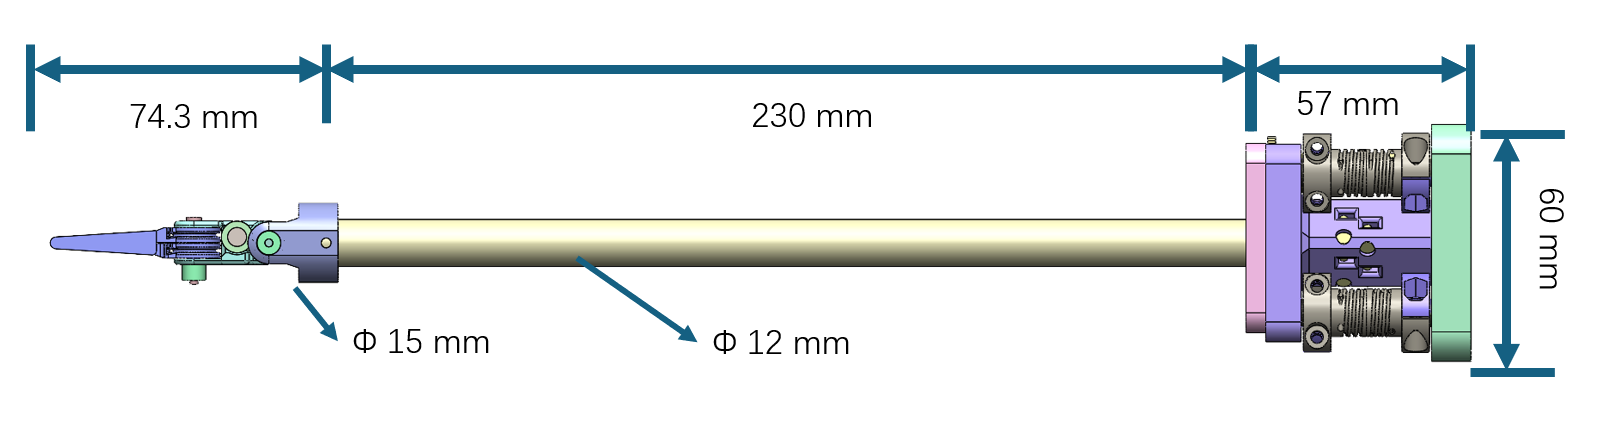
\includegraphics[width=\linewidth]{Figures/Chapter4/Winding_Size.png}

    \caption{Winding mechanism and shaft layout. The 250\,mm carbon tube provides the main shaft structure, while internal Teflon guidance and paired reel components maintain the cable route and tension.}
    \label{fig:winding_exploded}
\end{figure}

The key to ensuring effective operation of this belt-like linkage is sustained cable tension. To achieve this, the reel assembly is split into two distinct components, each dedicated to one cable. These two reel pieces are mounted on the same shaft and are designed to rotate in opposite directions relative to each other. This counter-rotation ensures that one cable is wound while the other is unwound during actuation, maintaining constant tension across the system.

To prevent slippage and undesired loosening of the cables during operation, one-way bearings are incorporated into the reel mechanism. As the name implies, these bearings permit free rotation in one direction while locking in the opposite direction. This feature is critical for preserving tension integrity, especially during transitions in motor direction or under varying load conditions. The use of one-way bearings enhances system reliability, improves motion accuracy, and minimizes the need for manual tension adjustments.

The reel diameter is matched to the tip rotation-axis diameter at 11\,mm, producing a nominal 1:1 displacement relationship between reel rotation and the corresponding tip-side cable displacement. This geometric matching simplifies command mapping because the controller does not need to compensate for an additional reel-to-tip radius ratio. For the roll transmission at the tip, the driving gear has 35 teeth and the driven gear has 65 teeth. The resulting angular reduction is $35/65$, while the ideal torque is increased by approximately $65/35$ before frictional losses. This ratio was selected to improve fine angular resolution and keep the quick-swap distal module compact.

\subsubsection{Actuator-to-Cable Force Mapping}
The reel geometry provides a direct way to estimate the upper-bound cable load generated by the output servos. The STS3032 stall torque is specified as approximately $4.5\,\mathrm{kg\,cm}$. Converting this value into SI units gives
\[
\tau_{stall}=4.5 \times 9.80665 \times 10^{-2}
\approx 0.441\,\mathrm{N\,m}
=441\,\mathrm{N\,mm}.
\]
With the reel diameter set to 11\,mm, the nominal reel radius is $r=5.5\,\mathrm{mm}$. Neglecting friction and cable compliance, the maximum single-cable tension that can be produced at the reel is therefore
\[
F_{cable,max}=\frac{\tau_{stall}}{r}
=\frac{441}{5.5}
\approx 80.2\,\mathrm{N}.
\]
This value is not intended to represent the normal continuous operating tension. It is an upper-bound estimate used for structural checking and safety-limit reasoning. In normal operation, the firmware commands position and speed within a limited range and avoids sustained stall conditions. Nevertheless, the stall-torque-derived load is useful because it defines the most severe actuator-driven load that the distal parts may experience before controller intervention.

The selected 0.5\,mm 7$\times$37 tungsten cable has a rated breaking force of 501.7\,N. Comparing this rating with the ideal stall-derived cable tension gives a cable-side strength margin of approximately
\[
SF_{cable}=\frac{501.7}{80.2}\approx 6.26 .
\]
This margin is evaluated only against axial cable breaking strength. It does not include losses from bending fatigue, local abrasion, knotting or crimp termination, pulley groove quality, or repeated sterilization and cleaning processes. For this reason, the cable is treated as structurally sufficient for prototype validation, but future versions should still include cycle-life tests under representative routing and tension profiles.

In addition to the axial strength margin, extra cable length was reserved for assembly and pretensioning. The prototype keeps approximately two additional turns on the 11\,mm-diameter reel, corresponding to an installation allowance of
\[
l_{allowance}=2\pi D=2\pi(11)\approx 69.1\,\mathrm{mm}.
\]
This reserved length is used to mount the cable securely and to tighten the opposing reel during setup. It should be interpreted as an installation and pretensioning allowance, not as an additional mechanical strength safety factor. The axial safety factor above describes the cable's load capacity under the stall-torque-derived tension, whereas the two-turn allowance improves assembly robustness and makes it easier to remove slack from the antagonistic cable pair.

\begin{table}[htbp]
    \centering
    \caption{Nominal actuator-to-cable force estimates for the output drive}
    \label{tab:actuator_cable_force}
    \small
    \setlength{\tabcolsep}{4pt}
    \begin{tabular}{@{}p{0.22\linewidth} p{0.22\linewidth} p{0.46\linewidth}@{}}
        \toprule
        Quantity & Value & Interpretation \\
        \midrule
        STS3032 stall torque & $4.5\,\mathrm{kg\,cm}$ & Maximum actuator torque before controller derating or protection \\
        Reel diameter & $11\,\mathrm{mm}$ & Matches the tip rotation-axis diameter for a nominal 1:1 displacement relationship \\
        Ideal maximum cable tension & $80.2\,\mathrm{N}$ & Upper-bound tension from stall torque and 5.5\,mm reel radius \\
        Tungsten cable breaking force & $501.7\,\mathrm{N}$ & Axial rating of the selected 0.5\,mm 7$\times$37 cable \\
        Cable axial safety margin & $6.26$ & Margin against ideal stall-derived cable tension before routing and termination effects \\
        Installation allowance & $\approx69.1\,\mathrm{mm}$ & Two reserved turns on the 11\,mm reel for mounting and opposing-reel pretensioning \\
        \bottomrule
    \end{tabular}
\end{table}

The same calculation also explains why the FEA load cases were derived from the actuator torque rather than from an arbitrary external force. The servo defines the largest force that the cable transmission can inject into the distal mechanism under normal electrical power. Because the reel and tip share the same nominal diameter, the cable displacement at the reel can be interpreted directly as cable displacement at the tip before friction and elastic stretch are considered. This makes the structural model traceable from motor specification to cable tension and then to local component loading.

For the roll transmission, the 35-tooth driving gear and 65-tooth driven gear modify the angular and torque relationship. Ideally, the output roll angle is
\[
\theta_{roll,out}=\frac{35}{65}\theta_{roll,in},
\]
while the torque available at the driven gear is increased by the inverse ratio,
\[
\tau_{roll,out}\approx \frac{65}{35}\tau_{roll,in}.
\]
This reduction is useful for handheld manipulation because the roll axis benefits from fine angular resolution and stable holding behavior. The penalty is that the input motor must rotate through a larger angular range to generate the same distal roll angle. Since the STS-series servos can be commanded precisely in position and speed, this penalty is acceptable for the current prototype.

\subsubsection{Cable Displacement and Motion Resolution}
The matched reel and tip diameter also provides a simple displacement model. For a reel radius $r$, a motor rotation of $\Delta\theta$ produces an ideal cable displacement
\[
\Delta l = r\Delta\theta,
\]
where $\Delta\theta$ is expressed in radians. With $r=5.5\,\mathrm{mm}$, one degree of servo rotation corresponds to
\[
\Delta l_{1^\circ}=5.5\frac{\pi}{180}
\approx 0.096\,\mathrm{mm}.
\]
This sub-0.1\,mm nominal cable-displacement increment is sufficient for fine command mapping at the prototype level. Actual distal motion resolution will be lower because of cable stretch, guide friction, backlash in the reel assembly, gear clearance, and servo quantization. However, the geometric relationship provides a useful baseline for firmware scaling and calibration.

In the paired-cable arrangement, each controlled degree of freedom can be represented by an antagonistic displacement pair:
\[
\Delta l_+ = r\Delta\theta,\qquad
\Delta l_- = -r\Delta\theta .
\]
The first cable is shortened while the second cable is recovered by the same nominal amount. This pairing is the reason the mechanism can transmit motion bidirectionally even though a cable can only carry tensile load. The design objective is not to keep the individual cable lengths fixed, but to keep their sum and pretension within a useful range:
\[
l_+ + l_- \approx constant,\qquad
T_{min}<T_+,T_-<T_{max}.
\]
Here $T_{min}$ is the minimum tension required to avoid slack and delayed response, while $T_{max}$ is the maximum safe tension set by the cable, distal components, actuator load, and target tissue or object.

\begin{table}[htbp]
    \centering
    \caption{Transmission relationships used for control interpretation}
    \label{tab:transmission_relationships}
    \small
    \setlength{\tabcolsep}{4pt}
    \begin{tabular}{@{}p{0.24\linewidth} p{0.20\linewidth} p{0.48\linewidth}@{}}
        \toprule
        Relationship & Expression & Design meaning \\
        \midrule
        Cable displacement & $\Delta l=r\Delta\theta$ & Converts servo rotation into linear tendon motion \\
        One-degree increment & $\Delta l_{1^\circ}\approx0.096\,\mathrm{mm}$ & Baseline command resolution at the 11\,mm reel diameter \\
        Antagonistic pair & $\Delta l_+=-\Delta l_-$ & Maintains bidirectional actuation through paired cables \\
        Roll gear ratio & $\theta_{out}=35\theta_{in}/65$ & Improves roll resolution and holding torque \\
        Useful tension window & $T_{min}<T<T_{max}$ & Prevents both slack and overload \\
        \bottomrule
    \end{tabular}
\end{table}

This analysis is intentionally first-order. It does not attempt to model the full nonlinear friction and compliance of the cable path. Instead, it defines the nominal relationships used to choose hardware dimensions and firmware gains. More accurate compensation would require measuring cable tension and distal pose over repeated trajectories, then identifying hysteresis parameters for each cable route. That work is beyond the scope of the present prototype but follows naturally from the framework established here.

\subsection{Motor Arrangement and Quick-Swap Mechanism}

As previously discussed, the STS3032 servos are employed as the driving motors for the cable reels. In practical surgical scenarios, various end-effector tips are often required throughout a single procedure. To accommodate this need, a quick-swap system has been integrated into the design, allowing for rapid and secure tip replacement without compromising system integrity.

To achieve a compact form factor suitable for handheld operation, the four motors are arranged in a rotationally symmetric pattern within the main housing. This layout optimizes spatial efficiency while maintaining sufficient clearance for motor power and communication cables, thereby preventing interference and ensuring reliable connectivity.
\begin{figure}[htbp]
    \centering
    \begin{subfigure}[b]{0.7\linewidth}
        \centering
        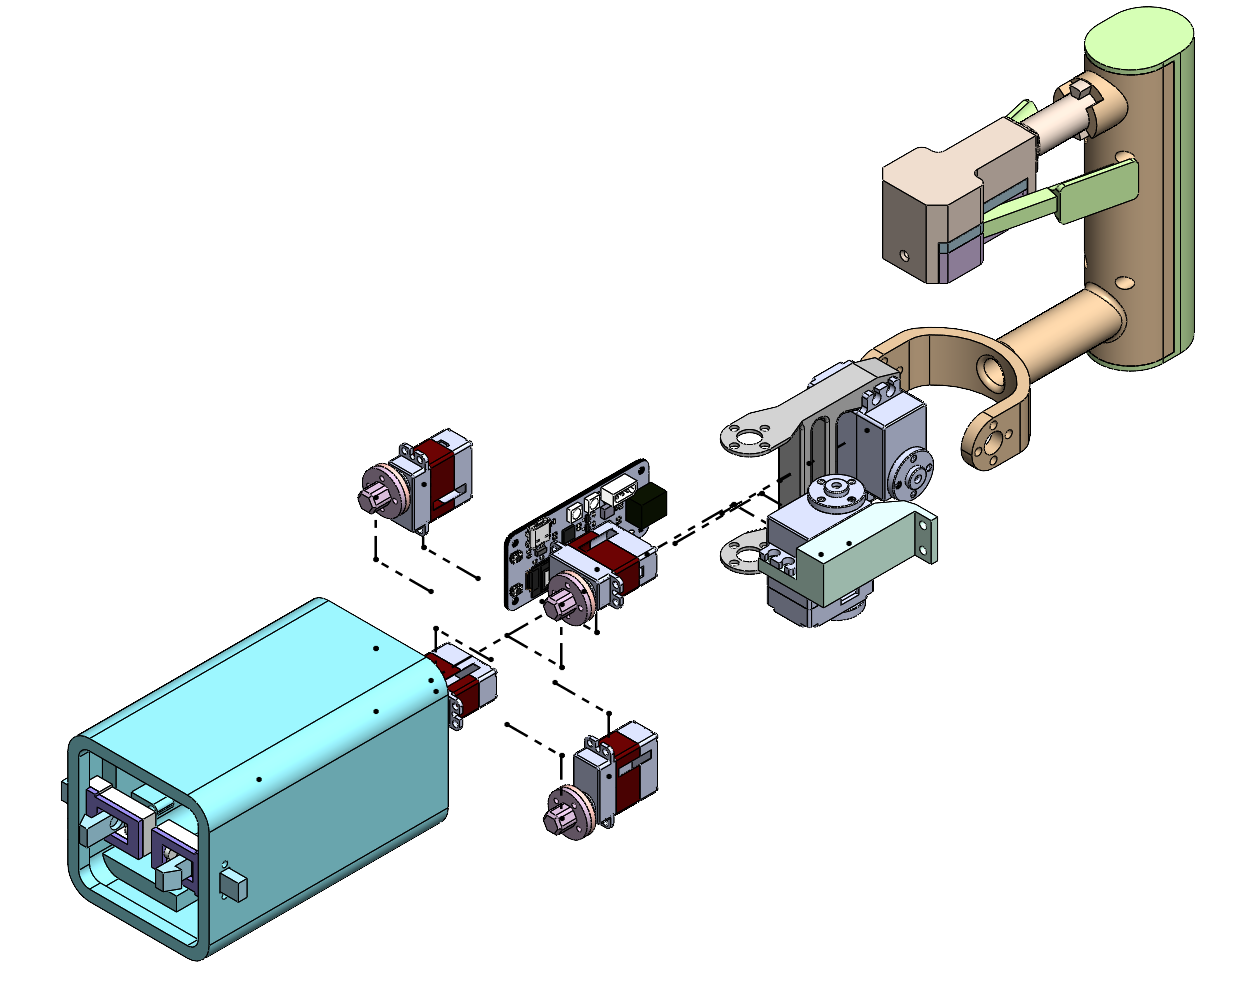
\includegraphics[width=\linewidth]{Figures/Chapter4/Main_Frame_ExplView_Iso.png}
        \caption{Exploded isometric view}
    \end{subfigure}

    \vspace{0.5em}

    \begin{subfigure}[b]{0.7\linewidth}
        \centering
        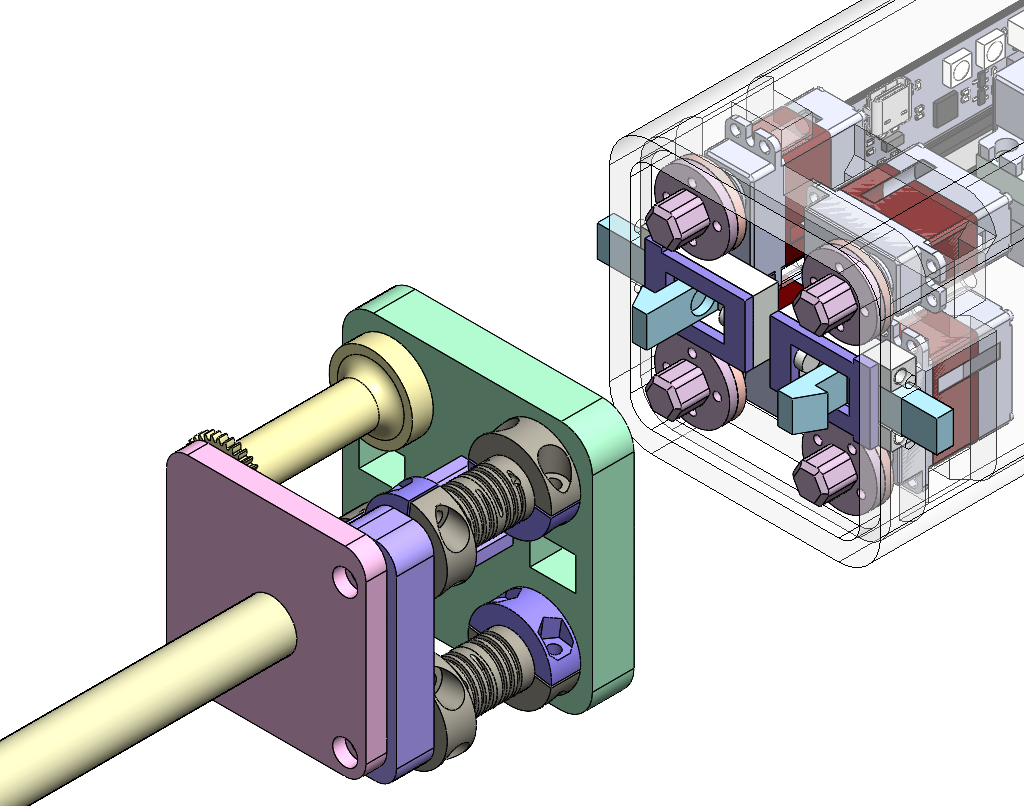
\includegraphics[width=\linewidth]{Figures/Motor Arrangement.png}
        \caption{Motor arrangement and quick-swap interface}
    \end{subfigure}
    
    \caption{Motor arrangement and quick-swap mechanism in the proximal frame. The output servos are packaged around the detachable shaft interface to preserve cable alignment while enabling tool exchange.}
    \label{fig:85}
\end{figure}
The quick-swap mechanism incorporates a user-friendly yet secure attachment scheme. Press-activated hooks are mounted within the main frame, enabling tool-free engagement and release. To attach a tip module, the user simply aligns and applies gentle pressure until the hooks audibly lock into place. For disengagement, bilateral release buttons must be depressed simultaneously while withdrawing the module. This dual-action release strategy prevents accidental detachment during operation, enhancing safety, while minimizing the number of steps required for module exchange.

This design ensures a robust mechanical and electrical connection during use, maintaining precise cable alignment and tension integrity while facilitating efficient tool interchange in time-sensitive surgical environments.

\subsection{Input Design}

The input module is designed to intuitively capture the user’s hand and finger motions with high precision and minimal latency. By integrating two STS3009 servos and two AS5600 magnetic encoders, the system is capable of sensing four degrees of freedom (DOFs): two DOFs from the wrist movement—yaw and pitch—and two DOFs from the fingers, namely roll and open/close actuation.

The wrist motions are translated through a dual-axis gimbal-like mechanism, where the STS3009 servos provide both actuation force and preliminary positional feedback. Fine rotational movements in yaw and pitch are accurately detected and relayed to the control system, enabling responsive and natural manipulation of the end-effector.
\begin{figure}[htbp]
    \centering
    \begin{subfigure}[b]{0.47\linewidth}
        \centering
        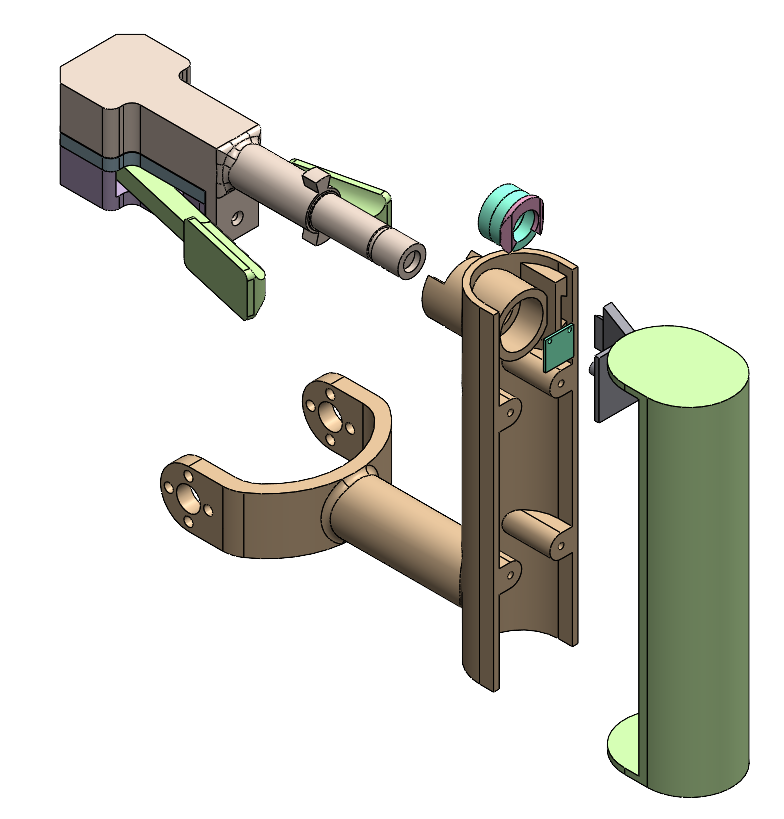
\includegraphics[width=\linewidth]{Figures/Chapter4/Input_Handle_ExplView_Iso.png}
        \caption{Input handle assembly}
    \end{subfigure}
    \hfill
    \begin{subfigure}[b]{0.47\linewidth}
        \centering
        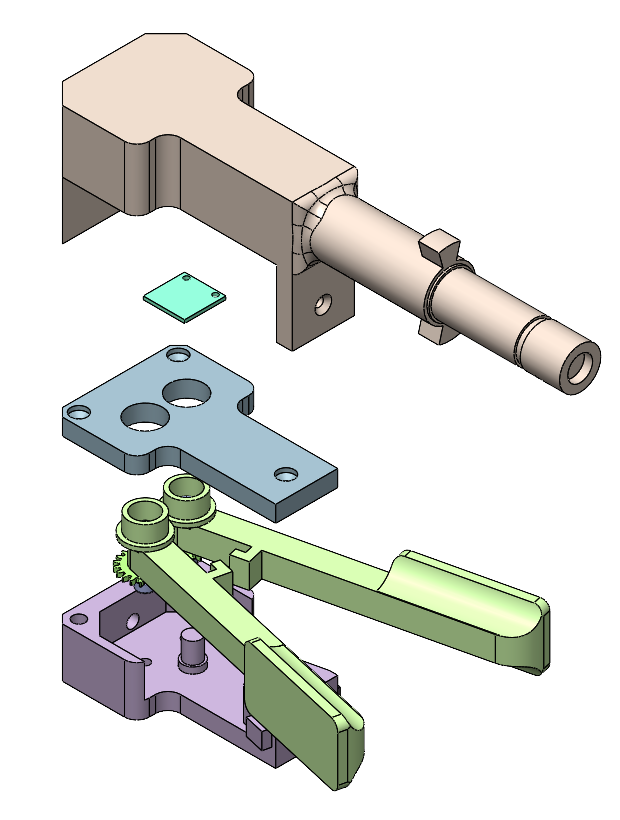
\includegraphics[width=\linewidth]{Figures/Chapter4/Pinch_ExplView_Iso.png}
        \caption{Pinch module}
    \end{subfigure}
    \caption{Input module design. Wrist pitch and yaw are captured through the STS3009-supported input handle, while roll and open/close commands are sensed by AS5600 encoders in the finger module.}
    \label{fig:86}
\end{figure}
Finger actions are captured using the high-resolution AS5600 encoders, which detect both the rolling gesture and the degree of opening or closing of the fingers. Specifically, the open/close mechanism is implemented as an interchangeable module, allowing customization based on user preference or task requirements. The lever length and rebound force can be easily adjusted or swapped, facilitating ergonomic adaptability and reducing user fatigue during prolonged operations.

This modular and sensor-rich input design ensures that the system can accommodate a wide range of hand sizes and operating styles while maintaining accurate and reliable motion mapping between the user and the instrument.

The project aims to implement a da Vinci–style surgical instrument claw effect using a compact 4-DOF hardware architecture: a 3-DOF manipulator arm plus a single gripper open/close degree of freedom. The system input is provided by the handle as three rotational joint angles and one gripper opening angle.

Since the manipulator itself has only three actual mechanical degrees of freedom, it cannot realize an arbitrary rotation axis in space. A specified direction in space requires three independent pose parameters, and a stable pose also consumes three degrees of freedom. This makes the system inherently over-constrained if arbitrary axis rotation is demanded. In contrast, the da Vinci system achieves effective 6-DOF stabilized control by using a larger arm to drive a smaller wristed arm in coordinated motion. Under the hardware constraints of this project, that six-degree-of-freedom stabilization strategy is not considered.

Instead, the control design adopts a decoupled attitude mapping. The coordinate system is defined using Euler angles to describe the desired end-effector orientation. The input attitude from the handle is mapped linearly to the output attitude of the manipulator, subject to the arm's three-degree-of-freedom limitations.


\subsection{Denavit–Hartenberg Coordinate Frames}
The coordinate frames are established using standard Denavit–Hartenberg conventions, as shown in Figures~\ref{fig:dhcord} and~\ref{fig:dhcord1}. The manipulator consists of three rotary joints, with the following D-H parameters:

\begin{table}[htbp]
    \centering
    \caption{Denavit–Hartenberg parameters for the 3-DoF manipulator}
    \label{tab:dhparams}
    \begin{tabular}{c c c c c l}
        \toprule
        Link & $\theta_i$ & $d_i$ & $a_i$ & $\alpha_i$ & Remarks \\
        \midrule
        1 & \(\theta_1\) & 0 & 0 & \(-90^\circ\) & Base rotation \\
        2 & \(90^\circ - \theta_2\) & 0 & \(-a_2\) & \(90^\circ\) & Upper arm rotation \\
        3 & \(\theta_3 - 180^\circ\) & 0 & \(a_3\) & 0 &  \\
        \bottomrule
    \end{tabular}
\end{table}

The following rotation matrix describes the end-effector orientation:

\[
A_1 =
\begin{bmatrix}
c_1 & 0 & -s_1 & 0 \\
s_1 & 0 & c_1 & 0 \\
0 & -1 & 0 & 0 \\
0 & 0 & 0 & 1
\end{bmatrix},
\]

\[
A_2 =
\begin{bmatrix}
s_2 & 0 & c_2 & -a_2 s_2 \\
c_2 & 0 & -s_2 & -a_2 c_2 \\
0 & 1 & 0 & 0 \\
0 & 0 & 0 & 1
\end{bmatrix},
\]

\[
A_3 =
\begin{bmatrix}
-c_3 & -s_3 & 0 & -a_3 c_3 \\
s_3 & -c_3 & 0 & a_3 s_3 \\
0 & 0 & 1 & 0 \\
0 & 0 & 0 & 1
\end{bmatrix}
\]
The end-effector pose is governed by the following equations:
\begin{align*}
P_x &= c_1 s_2(-a_3 c_3) + (-s_1)(a_3 s_3) + c_1 c_2(0) + (-a_2 c_1 s_2) \\
& \rightarrow P_x= -a_3 c_1 s_2 c_3 - a_3 s_1 s_3 - a_2 c_1 s_2 \\
P_y &= s_1 s_2(-a_3 c_3) + c_1(a_3 s_3) + s_1 c_2(0) + (-a_2 s_1 s_2) \\
& \rightarrow P_y= -a_3 s_1 s_2 c_3 + a_3 c_1 s_3 - a_2 s_1 s_2 \\
P_z &= -c_2(-a_3 c_3) + 0(a_3 s_3) + s_2(0) + a_2 c_2 \\
& \rightarrow P_z= a_3 c_2 c_3 + a_2 c_2
\end{align*}
The orientation of the end effector can also be expressed through the base axis direction vectors shown in Table~\ref{tab:axisdir}.

\begin{table}[htbp]
\centering
\caption{End-effector base-axis direction vectors}
\label{tab:axisdir}
\begin{tabular}{|l|l|l|l|}
\hline
\textbf{Direction} & \textbf{X-axis  ($n$)} & \textbf{Y-axis  ($o$)} & \textbf{Z-axis  ($a$)} \\
\hline
Base X-axis & $-c_1 s_2 c_3 - s_1 s_3$ & $-c_1 s_2 s_3 + s_1 c_3$ & $c_1 c_2$ \\
\hline
Base Y-axis & $-s_1 s_2 c_3 + c_1 s_3$ & $-s_1 s_2 s_3 - c_1 c_3$ & $s_1 c_2$ \\
\hline
Base Z-axis & $c_2 c_3$ & $c_2 s_3$ & $s_2$ \\
\hline
\end{tabular}
\end{table}

\begin{figure}[htbp]
    \centering
    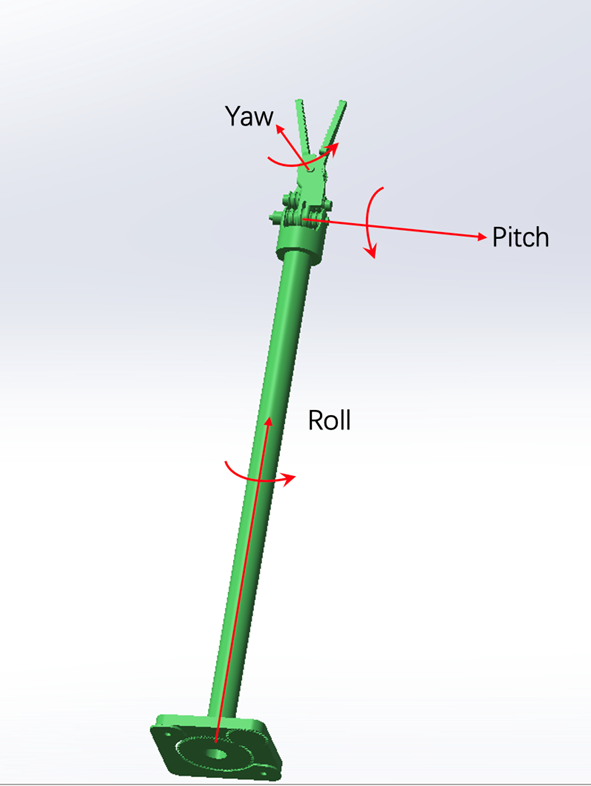
\includegraphics[width=0.7\linewidth]{Figures/DH cord1.png}
    \caption{Denavit–Hartenberg coordinate frame definition for the manipulator}
    \label{fig:dhcord}
\end{figure}

\begin{figure}[htbp]
    \centering
    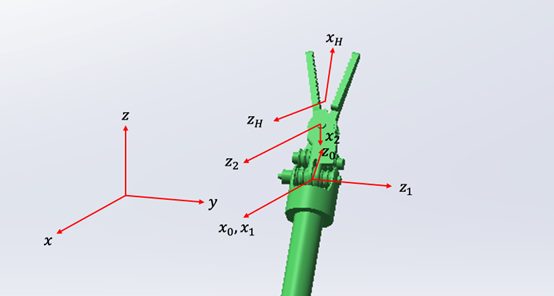
\includegraphics[width=0.8\linewidth]{Figures/DH cord.png}
    \caption{Alternative view of the D-H coordinate frames and joint axes}
    \label{fig:dhcord1}
\end{figure}

\subsection{System Architecture and Data Flow}
The control system is implemented on an ESP32 microcontroller running FreeRTOS, enabling real-time processing of sensor inputs and actuator commands. The architecture follows a cyclic loop structure, as illustrated in the firmware code, where sensor feedback is continuously acquired, processed, and translated into motor commands.

At the core of the system is a feedback loop that reads position, speed, load, voltage, temperature, and current from eight Feetech STS-series servos via UART communication. This multi-modal feedback provides the foundation for state estimation and control. The input module captures user intent through four degrees of freedom: wrist yaw, pitch, roll, and gripper opening/closing, using AS5600 magnetic encoders and STS3009 servos for precise motion detection.

The overall control pipeline is organized into four layers. The first layer is the sensing layer, where the AS5600 encoders and servo feedback registers are sampled. The second layer is the intent-estimation layer, where raw input angles are converted into centered, filtered, and range-limited user commands. The third layer is the command-mapping layer, where the desired roll, pitch, yaw, and open/close commands are transformed into individual output-servo setpoints. The fourth layer is the actuator layer, where the STS3032 servos execute the command while returning load and state information for monitoring.

\begin{table}[htbp]
    \centering
    \caption{Control-layer organization of the handheld instrument}
    \label{tab:control_layers}
    \begin{tabular}{p{0.22\linewidth} p{0.32\linewidth} p{0.30\linewidth}}
        \toprule
        Layer & Main function & Representative signals \\
        \midrule
        Sensing & Acquire raw input and actuator states & AS5600 angle, servo position, speed, load, voltage, temperature, current \\
        Intent estimation & Center, scale, filter, and limit the user's motion & Roll, pitch, yaw, and gripper-opening commands \\
        Command mapping & Convert user commands into output-axis setpoints & Four STS3032 position targets and motion limits \\
        Actuation and monitoring & Execute commands and detect abnormal states & Servo enable/unload state, load threshold, communication status \\
        \bottomrule
    \end{tabular}
\end{table}

This layered structure is important because it separates user-interface behavior from distal tool behavior. The handle may be redesigned in future versions without changing the output transmission model, provided that it still supplies normalized roll, pitch, yaw, and open/close commands. Similarly, the distal tool can be replaced through the quick-swap interface as long as its cable routing and command scaling remain compatible with the actuator layer. This modularity supports the broader thesis goal of applying tendon-driven design principles across multiple mechanical embodiments.

\subsection{Intent Estimation and Command Mapping}
User inputs are mapped from encoder readings to angular commands. The firmware calculates roll, pitch, yaw, and gripper commands by scaling encoder positions relative to a midpoint. For instance, $roll_cmd$ is derived from the difference between encoder p8 and the midpoint, scaled to degrees. These commands are then transformed into servo-specific inputs, accounting for mechanical ratios and phase offsets to ensure coordinated motion.

The transformation incorporates kinematic considerations, such as the differential yaw control for the gripper jaws, where $s3\_yaw\_right$ and $s4\_yaw\_left$ are adjusted based on $yaw\_in$ and $gripper\_cmd$ to achieve symmetric or asymmetric grasping.

To robustly infer operator intent in the presence of noise and delay, an Extended Kalman Filter (EKF) can be integrated as a future enhancement. The EKF would fuse sensor inputs from AS5600 encoders, motor encoders, and optional inertial measurements from an IMU module. It maintains estimates of finger poses, wrist orientation, and cable tensions, enabling predictive control and improved stability during rapid transitions. This probabilistic approach handles uncertainties in sensor readings, providing smoother and more reliable command generation compared to the current direct mapping.

In the current prototype, the direct mapping can be written as a normalized affine transformation. For an input sensor reading $q_i$, the corresponding command is
\[
u_i = k_i(q_i-q_{i,0}),
\]
where $q_{i,0}$ is the neutral reference measured during homing and $k_i$ is the command gain selected for that degree of freedom. The command is then saturated:
\[
u_i^{sat}=\mathrm{clip}(u_i,u_{i,min},u_{i,max}).
\]
The saturation step is not only a software convenience. It is a safety mechanism that prevents the handle from commanding cable travel beyond the mechanically validated range of the reel, guide tube, pulley, and distal joint.

The four output commands are intentionally decoupled at the operator level:
\[
\mathbf{u}=
\begin{bmatrix}
u_{roll} & u_{pitch} & u_{yaw} & u_{grip}
\end{bmatrix}^T .
\]
They are then mapped into motor targets:
\[
\mathbf{m}=M\mathbf{u}+\mathbf{m}_0 ,
\]
where $\mathbf{m}$ contains the four STS3032 target positions, $M$ is a sign-and-scale matrix determined by cable routing direction and gear ratio, and $\mathbf{m}_0$ contains the neutral motor positions. In the simplest case, each row of $M$ contains only one dominant nonzero term. In practice, the jaw and yaw axes may be coupled because the same distal geometry contributes to both lateral orientation and symmetric jaw motion. The firmware therefore applies sign offsets so that symmetric closing commands move both jaws together, while yaw commands create differential motion.

\begin{table}[htbp]
    \centering
    \caption{Command interpretation for the four output degrees of freedom}
    \label{tab:command_mapping}
    \begin{tabular}{p{0.18\linewidth} p{0.24\linewidth} p{0.38\linewidth}}
        \toprule
        Command & Primary input source & Output interpretation \\
        \midrule
        Roll & AS5600 roll encoder & Rotates the distal tool through the 35:65 gear transmission \\
        Pitch & STS3009-supported wrist input & Bends the distal tool in the pitch plane through an antagonistic cable pair \\
        Yaw & STS3009-supported wrist input & Produces lateral distal orientation through differential cable motion \\
        Open/close & AS5600 pinch encoder & Controls jaw aperture and grasping tension \\
        \bottomrule
    \end{tabular}
\end{table}

Several practical issues arise in this mapping. First, the neutral position must be repeatable. If the user powers on the device while the handle is displaced, the controller may interpret a biased input as the center position. The startup routine therefore moves the servos to known neutral positions and records sensor baselines before enabling full output motion. Second, the command gain must be conservative enough to prevent sudden distal motion, especially near the limits of the jaw and pitch axes. Third, the sign convention must be verified physically after every cable rerouting or tip replacement, because crossing a cable or reversing a reel direction changes the relationship between motor rotation and distal motion.

\subsection{Low-Level Actuation and Tension Management}
Actuation is handled through direct position control of the STS3032 servos for the output stage and STS3009 for input stabilization. The code implements a locking mechanism for the gripper motors: when the gripper is open beyond a threshold $(gripper_open = 5.0 degrees)$, the motors are unloaded to reduce power consumption and allow free motion; otherwise, they are locked to maintain tension.

This tension management is critical for cable-driven systems, preventing slack while enabling compliant interaction. The firmware uses the servo's built-in position mode with zero speed and acceleration for precise control, ensuring smooth transitions without oscillations.

For a tendon-driven tool, low-level control cannot be evaluated only by whether the servo reaches a target position. The control objective is to reach the target while maintaining the cable inside a useful tension range. A simple practical interpretation is:
\[
T_{min}<T(t)<T_{max},
\]
where $T_{min}$ prevents backlash and delayed response, while $T_{max}$ prevents cable damage, component yielding, motor overheating, and excessive tool force. Because the current prototype does not include direct inline cable-load cells at every tendon, the firmware uses servo load feedback as an indirect monitoring signal. This indirect signal is sufficient for prototype protection and debugging, but it is not a substitute for calibrated distal force sensing.

The control strategy therefore combines position commands with state-dependent enable and unload logic. When the gripper is open beyond the defined threshold, the controller can unload selected servos to avoid unnecessary cable tension and heat generation. When the gripper is closing or holding, the output servos are enabled so that the cable path remains tensioned and the jaws do not drift. This behavior is particularly important for surgical-style use because an unintended holding force could damage tissue, while an unintended release could cause loss of object control.

\begin{table}[htbp]
    \centering
    \caption{Representative tension-management states}
    \label{tab:tension_management_states}
    \begin{tabular}{p{0.20\linewidth} p{0.33\linewidth} p{0.31\linewidth}}
        \toprule
        State & Controller behavior & Purpose \\
        \midrule
        Open and idle & Selected motors unloaded or low-torque holding & Reduce heat and avoid unnecessary distal force \\
        Commanded motion & Position targets updated with speed limits & Produce smooth motion while avoiding sudden cable loading \\
        Grasp or hold & Motors enabled and position maintained & Preserve cable tension and jaw closure \\
        Overload indication & Stop, relax, or reject further closing command & Protect cable, distal parts, and target object \\
        Communication fault & Stop command update and enter error indication & Prevent uncontrolled motion under missing feedback \\
        \bottomrule
    \end{tabular}
\end{table}

The one-way bearings in the reel assembly complement the firmware strategy. Mechanically, they reduce the tendency for a cable to unwind when load direction changes or when the motor is temporarily unloaded. Electrically, the firmware avoids repeatedly driving the motor against the same holding load when mechanical retention is sufficient. This mechanical-electrical division of responsibility is useful in a handheld device because it reduces power consumption and heat while improving perceived stability.

\subsection{System Implementation and Details}
Safety is ensured through conditional motor unloading and error management. When feedback faults occur—such as communication dropouts—the system illuminates an error LED and stops execution. At startup, a homing routine moves the servos to their neutral positions, enabling the encoders to establish reference baselines.

While running, the lock/release mechanism functions as a safety measure: it relieves cable tension whenever the gripper is open, preventing unintended forces on tissue.

Visual and diagnostic feedback is delivered through a WS2812 LED strip and serial output. Error conditions activate red LEDs, whereas normal operation leaves the indicators off. Both USB and Bluetooth connectivity support data logging, facilitating offline analysis of control performance and user interactions.

The firmware communicates with servos via HardwareSerial at 500k baud and uses standard Serial for debugging. Motor commands are assembled using a custom protocol that includes unload/enable directives. The main loop executes roughly every 3~ms, striking a balance between system responsiveness and computational overhead.

This implementation embodies a practical tendon-driven control framework, translating high-level intentions into low-level actuation while emphasizing safety and usability within a compact, real-time system.

\subsubsection{Homing and Calibration Procedure}
The homing procedure establishes the mechanical and electronic zero state of the instrument. At power-on, the controller first checks communication with all STS-series servos and verifies that the AS5600 encoders return valid angular readings. The output servos are then moved to their neutral positions, and the input sensors are sampled to define the operator-center reference. This sequence prevents the system from immediately converting an arbitrary startup posture into a distal tool command.

Calibration is especially important because the cable transmission is not perfectly rigid. Small changes in cable pretension, guide-tube seating, reel assembly position, and quick-swap module alignment can shift the neutral distal pose. The prototype therefore treats neutral calibration as part of the operating procedure rather than as a one-time factory setting. After the tool module is inserted, the user can bring the handle to its neutral posture and allow the firmware to store the corresponding encoder baselines. The output motors then apply only limited holding torque until the command state is enabled.

\begin{table}[htbp]
    \centering
    \caption{Startup and calibration sequence}
    \label{tab:startup_calibration}
    \begin{tabular}{p{0.16\linewidth} p{0.44\linewidth} p{0.24\linewidth}}
        \toprule
        Step & Operation & Failure response \\
        \midrule
        Device check & Confirm servo communication and sensor readings & Enter error indication if feedback is missing \\
        Mechanical neutral & Move output servos to predefined neutral positions & Keep motors unloaded if motion is blocked \\
        Input baseline & Record AS5600 and STS3009 neutral readings & Reject commands until readings are stable \\
        Pretension check & Apply limited holding command and inspect response & Relax cable if load estimate is abnormal \\
        Enable control & Accept user roll, pitch, yaw, and grip commands & Continue monitoring load and communication \\
        \bottomrule
    \end{tabular}
\end{table}

This procedure also supports the quick-swap concept. If a distal module is exchanged, the controller does not assume that the previous neutral offset remains valid. Recalibration after module insertion reduces the risk of accumulating cable bias across tool changes. In a future clinical version, this procedure would need to be further constrained by sterilizable connectors, keyed mechanical alignment, and automated verification of tool identity.

\subsubsection{Fault Handling and Safety State Machine}
The safety logic can be represented as a state machine that limits how the device reacts to abnormal conditions. The normal operating state accepts user commands and updates servo targets. If the input command exceeds the allowed range, the controller clips the command rather than passing it directly to the output servo. If the servo load or temperature rises beyond an acceptable range, the controller can stop further closing motion, relax the corresponding cable, or enter a fault state depending on severity. If communication with a servo is lost, the system stops command updates and provides a visible error indication through the LED interface.

\begin{table}[htbp]
    \centering
    \caption{Safety-related events and controller responses}
    \label{tab:safety_events}
    \begin{tabular}{p{0.26\linewidth} p{0.34\linewidth} p{0.24\linewidth}}
        \toprule
        Event & Detection source & Response \\
        \midrule
        Command exceeds travel limit & Scaled input command after saturation check & Clip command to validated range \\
        Possible cable overload & Servo load feedback or abnormal holding demand & Stop closing or relax affected axis \\
        Servo communication fault & Missing or invalid UART response & Freeze command update and show error LED \\
        Startup bias & Input baseline unstable during homing & Delay enabling output motion \\
        Excessive heating risk & Servo temperature or prolonged high-load state & Reduce holding command or unload motor \\
        Quick-swap uncertainty & Module exchange or alignment disturbance & Require neutral recalibration \\
        \bottomrule
    \end{tabular}
\end{table}

The safety state machine is deliberately conservative. The prototype is intended to validate mechanism feasibility, not to maximize speed at the expense of controllability. Therefore, ambiguous states are treated as reasons to stop or relax motion rather than to continue driving the tendon path. This approach is consistent with the design philosophy of cable-driven medical tools, where the consequences of excessive force are more severe than the inconvenience of stopping a command.

\subsubsection{Control Limitations}
The present control implementation has several limitations. First, distal pose is inferred from motor position and transmission geometry rather than measured directly at the tool tip. As a result, cable stretch, friction, backlash, and guide-tube movement can create differences between commanded and actual pose. Second, load monitoring is indirect. Servo load feedback is useful for detecting abnormal trends, but it does not provide a calibrated measurement of cable tension or tissue force. Third, the current mapping is mostly linear. This is appropriate for a first prototype, but the real transmission is nonlinear because friction changes with bend angle, direction of motion, and cable normal force.

These limitations define the next control-development path. A more advanced version should add distal pose or force sensing, identify hysteresis maps for each cable route, and compensate for cable stretch under load. Repeated cyclic tests should be used to measure backlash, settling time, and drift. The current architecture is compatible with these future improvements because it already separates sensing, intent estimation, command mapping, and low-level actuation. The missing elements are therefore additional measurement channels and experimentally identified compensation parameters rather than a complete redesign of the control framework.
